\chapter{Implementation of Application Energy Monitoring}
\label{chapter:implementation}

\section{Introduction}
The functional design presented in Section V abstracts away implementation details, in order to concentrate on the essence of the problem and our solution.  In this section, we consider how to implement the functional design.
In order to both align with industrial practice and also simplify our implementation as much as possible, we have made a number of assumptions about the system being investigated:

\begin{itemize}
\item \emph{Containerisation} - we assume that all application elements which need to have energy usage estimated for them can be packaged in runtime containers - specifically Docker containers [REF].  Given the current wide industrial usage of Docker and its alignment with the microservice architectural style, we believe that this is an entirely realistic assumption.
\item \emph{Tracing} - we assume that all Application Service elements can participate in tracing of their requests and invocations and specifically that they can generate a Zipkin [REF] trace record stream.  Zipkin is widely adopted in industry (REF) and existing instrumentations exist for C\#, Go, Java and JavaScript, amongst others [REF].  We think this will cover most industrial cases.  In addition, Zipkin has been tightly integrated into a number of very widely used microservice frameworks, like Spring Boot [REF] and DropWizard [REF], which makes its use trivial for developers who are using a framework to create their services.  Therefore we do not believe that this assumption is likely to cause problems for the foreseeable future.
\item \emph{Architectural Description} - we assume that some of the structural aspects of the system that we need (service relationships in particular) are available via an architectural description that we assume is described using xADL [REF].  From an industrial perspective this is a less realistic assumption as few industrial projects use machine readable architectural descriptions of any sort and very few, if any, use xADL.  However we need this information for some of the calculations and so the architect does need to capture it and a notation is needed to achieve this. xADL is simple and practical and so while not part of current industrial practice, we do not believe that it will be a major problem and indeed could motivate industrial architects to create simple, useful, machine-readable architectural descriptions, which could be then used for other purposes too.  The implementation also isolates the xADL dependency in one module of the code and so could easily use alternative representations if xADL proves to be problematic.
\end{itemize}

The implementation design of the system is shown in the simple block diagram in Figure 3. The system elements filled with the fine dotted pattern are the elements of the application (Application Services, Black-Box Services and Asynchronout Processors), the system elements filled with the fine cross-hatching are data elements, while the Apollo Energy Estimator is filled with the light solid fill.  The unshaded elements are third party technologies which are reused unchanged as part of the implementation.

\begin{figure}
\centering
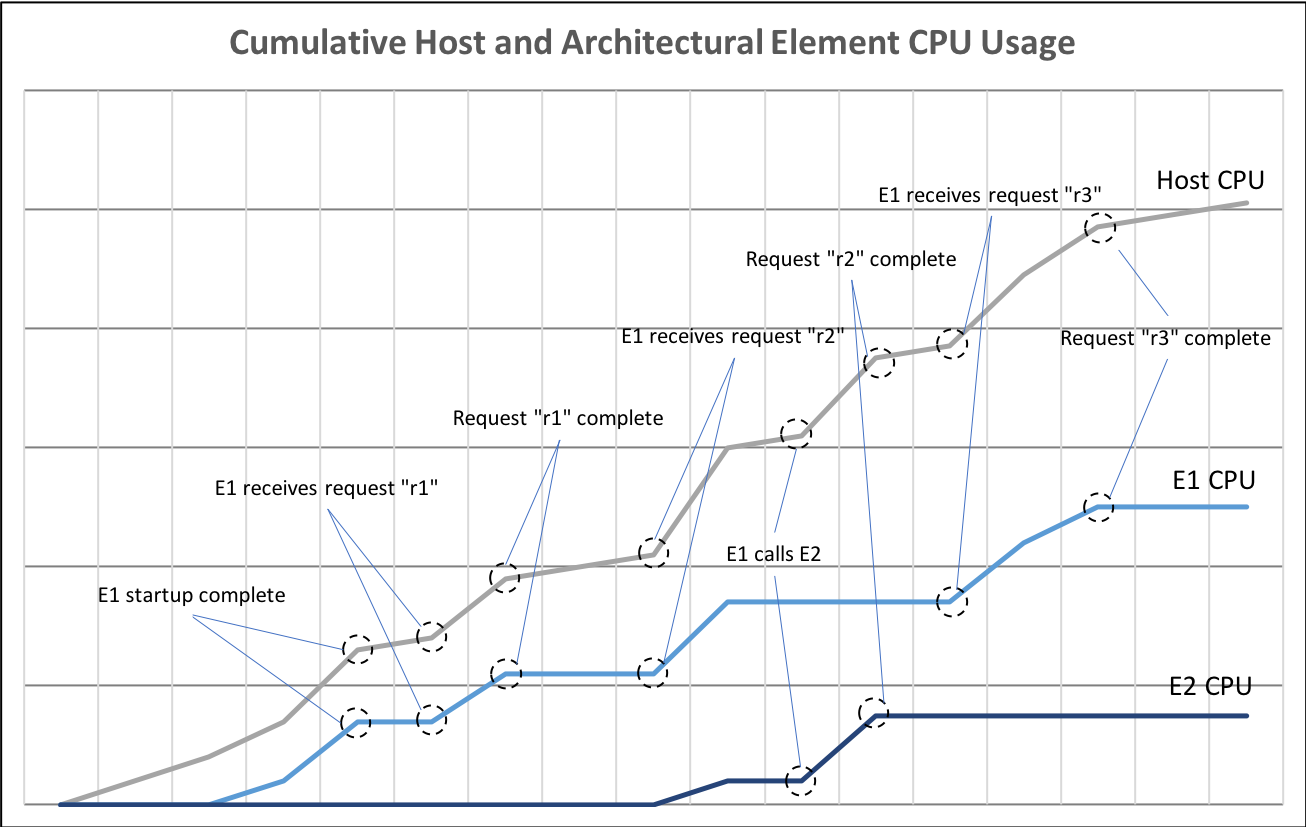
\includegraphics[width=1.0\textwidth]{Figures/estimating-energy-cpuusage}
\caption{Implementation of the Apollo Energy Estimator}
\label{figure:implementation}
\end{figure}

The significant third-party technologies used in this implementation are:
\begin{itemize}
\item Docker - as mentioned above, all application elements need to run within Docker containers.  This allows metadata about the elements to be retrieved and resource usage statistics to be gathered.
\item Zipkin - a trace of the invocations to and between application elements is required and as explained above, the Zipkin tracing system is used to achieve this.
\item Telegraf - the Docker platform produces a stream of resource usage statistics for the containers that it is executing.  The Telegraf agent [REF] collects these metrics and stores them in a timeseries database for easy retrieval.
\item InfluxDB - is used as the timeseries database for the Resource Usage Records.
\item xADL - as explained above, we need some structural information about the application to allow integration of energy estimations for untraceable elements.  xADL is the machine readable notation used for this.
\end{itemize}

The operation of the energy estimation system is similar to the simpler functional design explained earlier.  The elements of the system and the responsibilities of each and their key interactions are as follows:

\begin{itemize}
\item Application Service - represents the regular microservices that comprise the application under investigation.  The implementation of these services are under the control of the development team and they have the responsibility to generate Zipkin trace records (via the Zipkin Client library) to record their activity (although this will usually be achieved automatically through use of an application framework like Spring Boot).
\item Other Service - represents the services within the system which cannot be altered by the development team (“Blackbox Services”) or services which, although part of the system, do not take a direct part in request processing but are triggered as a side effect of it (“Asynchronous Processors”).  These system elements do not generate Zipkin traces.
\item Docker Container - the runtime container for all of the application system elements.   It provides isolation for the element within it and an interface to the Docker Runtime.
\item Docker Runtime - is the execution platform for the application system elements, through their use of containers.  The Docker Runtime is responsible for maintaining the topology of the Docker environment (e.g. which containers are running) and tracking resource utilisation of each container (CPU, memory, disk i/o and network i/o).  It streams the container level resource utilisation metrics to the Telegraf Server.
\item Zipkin Client - a client programming library used by Application Services to generate trace records and forward them to the Zipkin Server for storage.  The application code may invoke this library directly or it may be invoked automatically by an application framework like Spring Boot or Drop Wizard.
\item Zipkin Server - accepts incoming streams of trace records from application elements, stores them in the Trace Records database, and provides access to the records (although the records can also be accessed directly from the database, which is what we do in this case).
\item Trace Records - the database of trace records from Zipkin, recording application element activity.
Telegraf Server - an open source metrics collection agent, which accepts the stream of resource usage metrics from Docker and writes them to the Resource Usage Records database.
\item Resource Usage Records - a database of container level resource usage metrics, originally generated by the Docker Runtime.  This is ideally a timeseries database (we use InfluxDB) to allow efficient storage and retrieval of traces and spans by time range.
\item Docker Network Map - the Docker part of the system identifies architectural elements by container ID (which are large numbers) whereas the Zipkin part of the system has no visibility of container IDs and identifies architectural elements primarily by network address.  The Docker Network Map is a datastructure allowing a mapping between the two worlds, and is generated using the Docker “network inspect” command or API call.
\item xADL Architectural Description - as explained previously, in order to make a good estimation of energy usage, we need to be able to understand all of the architectural elements involved in a request.  Some form of machine readable architectural description is needed to provide this information and we have selected xADL as the notation for this, given its relative maturity, standard XML-based technology and tools.
\end{itemize}

Apollo Energy Estimator - is the calculator that produces the energy estimate for each request made to the system.  This architectural element implements the algorithm defined in Figure \ref{figure:implementation}. This means that it:

\begin{itemize}
\item Reads the Trace Records store to extract the Zipkin traces and spans.
\item For each trace that it finds, uses the Network Map to identify the containers that correspond to each trace and span that produced the traces and spans.
\item Reads the xADL Architectural Description to identify the other containers which the architect wishes to be included in the energy estimate for particular requests (based on the containers involved in processing each trace and the relationships between those containers and other containers found in the architectural description).
\item Using the container identities and the start and end times of the corresponding trace or span records, reads the Resource Usage Records store to find the CPU, memory and IO consumption of each container during the relevant time period. 
\item Sums the resource usage statistics for each trace and its child spans to produce total resource usage per request.
\item Calls the energy model to estimate energy usage for the resource usage for each request.
\end{itemize}

The result of this set of element interactions will be the Energy Estimator producing a set of energy consumption estimates for each of the trace records that it finds in the Trace Records store when it is run.

\section{Limitations of Apollo}

The design described in this paper has been validated via proof-of-concept implementations of each of its significant decisions and mechanisms, but not yet built.  Therefore the next step in the work is a full, robust implementation which can be utilised and validated to create a useful energy estimation mechanism.
The design described here is the first development of the ideas and has a number of limitations, which can be addressed in future work.

Our approach estimates energy usage for individual requests, by estimating the energy usage of each container as the request is processed.  This allows some degree of isolation as other workload which does not use these containers can be running in the application without it distorting the results.  For Application Service elements this is useful, as they are usually replicated for scalability reasons and so workload can run in the replicas that are not processing the request of interest.  However, care must be taken not to have workload running through shared services (such as databases) which would distort the energy estimation.  This is a limitation of the current version of the design. In practice, we believe that architects are likely to expect this constraint, as it is similar to the situation for other non-functional tests like performance and scalability.

The use of the architectural description data is somewhat unsatisfying as the rest of the inputs to the process are automatically generated.  The creation of the architectural description is a burden for the architect and could be performed incorrectly.  A more sophisticated tracing system, which can trace the activity of “black box” components could go some way to addressing this and could potentially be achieved by lower-level tracing in the operating system and network layer.

The system does not provide the architect with any visualisation or analytics view of the data in order to help draw insights from it.  While not the focus of this work, there are a number of well-known tools (such as Graphana) that could be used to create a visual interface for understanding the results of the analysis.

Third, the energy estimates for each trace and span are derived from sampled resource usage statistics for the corresponding container.  The sample times will very rarely align with the start and end times of the traces and spans and so estimates will need to be made, based on the samples available.  Depending on the sampling interval of the resource monitoring and the timing of the traces and spans, it is possible that the simple estimation approach we use could prove to be inaccurate (perhaps missing peaks and troughs between sample intervals).  The sample intervals we achieve in practice are short (TODO - HOW LONG?) and so we do not believe that this is a significant limitation, but does need to be monitored in practice.

\section{Summary}

